%\part{网络服务}

%\begin{frame}{网络服务}
%	\tableofcontents[currentsection]
%\end{frame}

\section{服务访问控制}

\begin{frame}{服务访问控制}

目标
\begin{itemize}
\item 理解服务是如何管理的
\item 了解服务的共同特性
\item 描述服务配置资源
\item 访问控制实现
\end{itemize}

\end{frame} 
\begin{frame}{init管理的系统资源}
\begin{itemize}
\item 服务监听在串口协议连接上

\begin{itemize}
\item 串口终端
\item 调制解调器(modem)
\end{itemize}
\item 配置文件 /etc/inittab
\item 调用命令rc来执行初始化脚本
\item 调用脚本开始X11 显示管理器
\item 提供respawn能力

\begin{itemize}
\item 1:2345:respawn:/sbin/mingetty tty1
\end{itemize}
\end{itemize}

\end{frame} 
\begin{frame}{服务管理}
\begin{itemize}
\item 一般指的是'System V' 或'SysV'

\begin{itemize}
\item 脚本层级结构由文件系统目录来组织
\item 服务可以激活也可以禁止
\end{itemize}
\item 通常都有服务配置文件
\item 大部分服务启动一个或多个进程
\item 命令由脚本“包裹”(wrap)
\item 服务由/etc/init.d/目录下的脚本管理
\item 举例

\begin{itemize}
\item /etc/init.d/network status
\item service network status
\end{itemize}
\end{itemize}

\end{frame} 
\begin{frame}{chkconfig}
\begin{itemize}
\item 管理服务在各运行级别上的限定
\item 希望启动时运行网络服务:\\
chkconfig network on
\item 并不修改当前服务的运行状态
\item 用于独立的服务
\item 可以被其他应用程序调用,包括rfsysv
\item 列出运行级别服务状态表,执行\\
chkconfig --list
\end{itemize}

\end{frame} 
\subsection{xinetd 服务}


\begin{frame}{xinetd管理的服务}
\begin{itemize}
\item 管理按需启动的服务,且使用较少或者使用时间短暂

\begin{itemize}
\item 需求不太频繁的服务
\item 基于主机的认证
\item 服务统计和日志记录
\item 服务IP重定向
\end{itemize}
\item 配置文件 /etc/xinetd.conf,/etc/xinetd.d/\emph{service}
\item 与libwrap.so 连接
\item 服务可以由chkconfig 控制\\
chkconfig telnet on
\end{itemize}

\end{frame} \begin{frame}{xinetd 缺省控制}

顶级配置文件--xinetd.conf

\verbatiminput*{/etc/xinetd.conf}


\end{frame} \begin{frame}{xinetd服务配置}

服务配置文件 /etc/xinetd.d/\emph{service}

/etc/xinetd.d/telnet

service telnet

\{

disable = yes

flags = REUSE

socket\_type = stream 

wait = no

user = root

server = /usr/sbin/in.telnetd

log\_on\_failure += USERID

\}


\end{frame} 
\begin{frame}{xinetd访问控制}
\begin{itemize}
\item 可以写在/etc/xinetd.conf中,也可以写在/etc/xinetd.d/目录下的文件中
\item 也可以使用的控制语句

\begin{itemize}
\item 允许 only\_from = \emph{客户端描述}
\item 拒绝 no\_access = \emph{客户端描述}
\item per\_source = \emph{数量}
\item access\_time = \emph{客户端描述}
\end{itemize}
\end{itemize}

\end{frame} 
\begin{frame}{/etc/sysconfig/ 文件}
\begin{itemize}
\item 某些服务需要该目录下的配置文件来确定服务如何运行

\begin{itemize}
\item named
\item sendmail
\item dhcpd
\item samba
\item init
\item syslog
\end{itemize}
\end{itemize}

\end{frame} 
\begin{frame}{服务和应用访问控制}
\begin{itemize}
\item 特定服务配置

\begin{itemize}
\item 像httpd,smbd,squid等守护进程,都提供了自身的安全机制
\end{itemize}
\item 通用配置

\begin{itemize}
\item 所有程序都和libwrap.so关联,使用通用的配置文件
\item 因为xinetd和libwrap.so关联,因此影响到它提供的服务
\item 检查主机和远程用户名
\end{itemize}
\end{itemize}

\end{frame} 
\subsection{网络实验}


\begin{frame}{实验I:浏览Xinetd服务}
\begin{description}
\item [{场景:}] 系统安装了telenet软件包,希望被xinetd超级守护进程管理。telnet服务在需要的时候变得有效,当没有用户连接时,系统中并不存在telnet进程
\item [{要求:}] 配置基于xinetd管理的telnet服务
\end{description}

\end{frame} 
\section{远程访问服务器}

\begin{frame}{运程访问服务器}

目标
\begin{itemize}
\item 理解openssh的安全特性
\item 通过openssh远程访问于数据传输
\item 理解远程图形化访问
\item 掌握VNC使用
\end{itemize}

\end{frame} 
\subsection{OpenSSH 概述}



\begin{frame}{OpenSSH 概述}
\begin{itemize}
\item OpenSSH替代之前常用的非安全网络通信程序
\item 提供用户和基于令牌的认证
\item 提供通过端口转发将非安全协议建立在隧道(tunnel)内的能力
\item 系统缺省配置(客户端,服务端)位于/etc/ssh
\end{itemize}

\end{frame} 
\begin{frame}{OpenSSH 认证}
\begin{itemize}
\item sshd守护进程能够利用几个不同的认证方法

\begin{itemize}
\item 密码(安全发送)
\item RSA/DSA 键
\item Kerberos
\item s/key和安全ID
\item 使用系统键值的主机认证
\end{itemize}
\end{itemize}

\end{frame} 
\begin{frame}{OpenSSH 服务器}
\begin{itemize}
\item 在网络系统里提供极大的数据安全

\begin{itemize}
\item 公/私钥 加密
\item 和早期的SSH行业版本兼容
\end{itemize}
\item 通过libwrap.so实现基于主机的安全
\end{itemize}

\end{frame} 
\begin{frame}{OpenSSH 服务一览}
\begin{itemize}
\item 类型:SysV管理的服务
\item 软件包:openssh,openssh-clients,openssh-server
\item 守护进程:/usr/sbin/sshd
\item 脚本:/etc/init.d/sshd
\item 端口:22(可配置)
\item 配置:/etc/ssh/{*},\$HOME/.ssh/
\item 相关:openssl,openssh-askpass,tcp\_wrappers
\end{itemize}

\end{frame} 
\subsection{OpenSSH 配置}



\begin{frame}{OpenSSH 服务配置}
\begin{itemize}
\item sshd 配置文件: /etc/ssh/sshd\_config
\item 可考虑的配置选项

\begin{itemize}
\item Protocol
\item ListenAddress
\item PermitRootLogin
\item Banner
\end{itemize}
\end{itemize}

\end{frame} 
\begin{frame}{OpenSSH 客户端}
\begin{itemize}
\item 安全shell会话

\begin{itemize}
\item ssh \emph{hostname}
\item ssh \emph{user@hostname}
\item ssh \emph{hostname remote-command}
\end{itemize}
\item 远程文件和目录安全拷贝

\begin{itemize}
\item scp\emph{ file user@host:remote-dir}
\item scp -r \emph{user@host:remote-dir localdir}
\end{itemize}
\item sshd提供的安全ftp

\begin{itemize}
\item sftp \emph{host}
\item sftp -C \emph{user@host}
\end{itemize}
\end{itemize}

\end{frame} 
\begin{frame}{应用:RPM}
\begin{itemize}
\item 文件一致性的两种实现
\item 已经安装的文件

\begin{itemize}
\item MD5 单向哈希(hash)
\item rpm --verify/-V \emph{package\_name}
\end{itemize}
\item 发行包文件

\begin{itemize}
\item GPG公钥签名
\item rpm --import /etc/pki/rpm-gpg/RPM-GPG-KEY-redflag{*}
\item rpm --checksig/-K \emph{package\_file\_name}
\end{itemize}
\end{itemize}

\end{frame} 
\subsection{VNC:虚拟网络计算}


\begin{frame}{VNC:Virutal Network Computing}
\begin{itemize}
\item 允许通过网络访问或者共享完整的桌面环境

\begin{itemize}
\item 作为纯粹的X链接占用带宽极少
\item 服务端

\begin{itemize}
\item 每个独立用户都可以启动vncserver命令启动vnc服务
\item 运行\$HOME/.vnc/xstartup运行vnc服务
\item 可以设定不同于系统帐号密码的密码
\item 通过/etc/init.d/vncserver可以自启动vnc服务
\end{itemize}
\item 客户端

\begin{itemize}
\item 使用vncviewer host:screen 连接远程机器
\item 同一主机通过唯一的屏幕号来区分
\item 支持通过ssh隧道来链接 vncviewer -via user@remote localhost:1
\end{itemize}
\end{itemize}
\end{itemize}

\end{frame} 
\section{网络域名服务}

\begin{frame}{网络域名服务(DNS)}

目标
\begin{itemize}
\item 理解主机名解析和在网络系统组织上的作用
\item 使用普通程序探索和校验DNS服务操作
\item 描述域名系统(Domain Name System,DNS)
\item 配置基本的DNS服务
\end{itemize}

\end{frame} 
\subsection{DNS 原理}


\begin{frame}{DNS 概述}
\begin{itemize}
\item 把主机名解析成IP地址(正向查找)
\item 把IP地址解析成主机名(反向查找)
\item 允许多台机器成为一个逻辑组

\begin{itemize}
\item hostname.doman.tld
\item hostname.subdomain.domain.tld
\end{itemize}
\item 每一个名字服务器响应名字空间的一部分,成为区(zone)
\item 名字服务起缓存应答
\end{itemize}



\end{frame} 
\begin{frame}{DNS特定的解析器}
\begin{itemize}
\item host

\begin{itemize}
\item 永远不读/etc/nsswitch.conf
\item 缺省情况下,查找/etc/resolv.conf文件里的nameserver和search行
\item 缺省是最小化输出
\end{itemize}
\item dig

\begin{itemize}
\item 永远不读/etc/nsswitch.conf
\item 缺省情况下,仅查找/etc/resolv.conf文件里的nameserver 行
\item 输出是RFC标准的zone文件格式,该格式用于DNS服务
\end{itemize}
\end{itemize}

\end{frame} 
\begin{frame}{dig跟踪DNS查询}
\begin{itemize}
\item dig + trace redflag-linux.com

\begin{itemize}
\item 读取 /etc/resolv.conf 来决定名字服务器
\item 查询根名字服务器
\item 逐级查询名字记录
\end{itemize}
\item 上述被称为迭代查询(iterative query)
\item 初步观察:

\begin{itemize}
\item 名字组织成倒立数结构,根(.)在顶端
\item 名字层次结构允许DNS跨组织边界
\item 全质量主机名(QFDN)以点(.)结尾
\end{itemize}
\end{itemize}

\end{frame} 
\begin{frame}{其他观察}
\begin{itemize}
\item 每一条应答记录是以资源记录(resource record)形式展现的
\item 每一个资源记录有5个域

\begin{description}
\item [{domain}] 查询的域或者子域
\item [{ttl}] 记录缓存的秒数
\item [{class}] 记录分类(通常是IN)
\item [{type}] 记录类型,比如A,NS
\item [{rdata}] domain映射的资源数据
\end{description}
\item 概念上讲,对一个域的查询,映射到rdata就是一个应答
\end{itemize}

\end{frame} 
\begin{frame}{邮件交换Mail Exchanger)查询}
\begin{itemize}
\item 一条MX记录映射域名到一台邮件服务器的完全合格域名(full-qualified domain name,FQDN)上
\item dig -t mx redflag-linux.com
\item 观察

\begin{itemize}
\item rdata 域被扩充,加入了一块额外的数据,称为优先级(priority)
\item 优先级可以看作是网络的距离,网络偏爱短路径
\item 为了避免额外的查询,域名服务器通常在MX记录里提供一个额外的和FQDN响应的A记录
\item MX记录以及和它关联的A记录组成了域的邮件服务
\end{itemize}
\end{itemize}

\end{frame} 
\begin{frame}{zone,domain,authoritative}
\begin{itemize}
\item 一个域(domain)包含一个完整的分级域名下层树
\item 一个区(zone)则是域的一部分,被一个具体详细的服务器所管理
\item 子域可以被授权成为附加的域
\item 一个区可以直接管理子域
\end{itemize}

\end{frame} 
\begin{frame}{host 探测DNS}
\begin{itemize}
\item 下面的命令,增加-v参数可以看到以zone文件格式输出
\item 跟踪:无效
\item 委派:host -rt ns google.com
\item 强制迭代:host -r google.com
\item 反向查询:host 74.125.53.100
\item MX 查询:host -t mx redflag-linux.com
\item SOA 查询:host -t soa redflag-linux.com
\item 区传送:host -t axfr redflag-linux.com 192.168.1.2 or\\
host -t ixfr=\emph{serial} redflag-linux.com. 192.168.1.2
\end{itemize}

\end{frame} 
\subsection{BIND 概述}


\begin{frame}{Berkely Internet Name Domain}
\begin{itemize}
\item 一般称为BIND,运行为 named
\item BIND是互联网上应用最广泛的DNS服务器

\begin{itemize}
\item 提供正向查询,反向查询,转发和缓存功能
\item DNS RFC规范的参考实现
\item 运行在chroot环境下
\item 能同时为不同的域充当主(master)服务器和辅助(slave)服务器
\end{itemize}
\end{itemize}

\end{frame} 
\begin{frame}{BIND服务一览}
\begin{itemize}
\item 类型:SysV 管理的服务
\item 包:bind,bind-utils,bind-chroot
\item 守护进程:/usr/sbin/named,/usr/sbin/rndc
\item 脚本:/etc/init.d/named
\item 端口:53(域),953(rndc)
\item 配置:{[}/var/named/chroot{]}/etc/named.conf,/var/named/{*},/etc/rndc.key
\item 相关包:caching-nameserver,openssl
\item /etc/sysconfig/named
\item named 进程被SysV脚本激活后,会根据此文件的参数决定运行参数
\end{itemize}

\end{frame} 
\begin{frame}{开始BIND}
\begin{itemize}
\item 安装相关软件包

\begin{itemize}
\item bind 核心二进制程序
\item bind-chroot 安全考虑
\item caching-nameserver 初始配置
\end{itemize}
\item 开始配置

\begin{itemize}
\item service named configtest
\item service named start
\item chkconfig named on
\end{itemize}
\item 处理基本的named配置
\end{itemize}

\end{frame} 
\subsection{BIND 配置}


\begin{frame}{/etc/named.conf}
\begin{itemize}
\item named.conf 是BIND使用的默认配置文件
\item 在每一次named启动与挂起时都会被读取
\item 一个简单的文本文件,其中记录的可以包括options(全局参数)、zone(区域定义)、access control lists (访问控制列表)等
\end{itemize}

\end{frame} 
\begin{frame}{option}
\begin{itemize}
\item 在/etc/named.conf的options段申明
\item 常用的参数包括

\begin{description}
\item [{directory}] 指定zone文件的存放位置
\item [{forwarders}] 指定其商机域名服务器
\item [{allow-query}] 指定允许向其提交请求的客户
\item [{allow-transfer}] 指定允许复制zone数据的主机
\end{description}
\end{itemize}

\end{frame} 
\begin{frame}{主域}


\begin{itemize}
\item 由一个zone段在/etc/named.conf中申明
\item type master;
\item file:存放该zone数据的文件名

\begin{itemize}
\item 必须存在于options段中提及的目录之下
\item 文件名可以随意
\end{itemize}
\item allow-update:允许动态更新该zone数据的客户机
\end{itemize}

\end{frame} 
\begin{frame}{从域}
\begin{itemize}
\item 由一个zone段在/etc/named.conf中申明
\item type slave;
\item master:指定其主域名服务器

\begin{itemize}
\item 对应的主域名服务器必须承认并存放有该区域的数据
\end{itemize}
\item file:本地用于存放zone数据的文件
\item 从域名服务器总是试图与其master联系并获取一份当前数据的副本
\end{itemize}

\end{frame} 
\begin{frame}{反向解析域}


\begin{itemize}
\item 域的名字必须用.in-addr.arpa来结尾
\item 由一个zone段在/etc/named.conf中宣告
\item 反解析域一般对应到一个具体的IP段
\item 反解析域同样可以配置为从域
\item 许多服务会尝试进行反解析
\end{itemize}



\end{frame} 
\begin{frame}{zone文件}
\begin{itemize}
\item 文件通常存放在/var/named目录下
\item 以\$TTL开头
\item ; 后面表示注释
\item 包含的资源记录

\begin{itemize}
\item A 名字到IP地址的映射
\item PTR IP地址到名字的映射
\item CNAME 创建别名
\item MX 邮件交换记录
\end{itemize}
\item FQDN必须以.结尾
\item 每一个在/etc/named.conf中定义的zone都应该对应一个具体的zone文件
\end{itemize}

\end{frame} 
\begin{frame}{(resource record)资源记录}
\begin{description}
\item [{SOA}] 定义起始授权
\item [{NS}] 指定域名服务器
\item [{MX}] 指定邮件服务器
\item [{A}] 将一个域名解析成其后的IP
\item [{CNAME}] 将一个域名设置为另一个域名的别名
\item [{PTR}] 将一个IP地址指向一个域名/主机名
\end{description}

\end{frame} 
\begin{frame}{SOA 记录}


\begin{itemize}
\item SOA(Start of Authroity):起始授权
\item 在每一个域文件中都应该有一个SOA段\\
@       IN      SOA     localhost. root.localhost.  (
\end{itemize}
                                      1997022700 ; Serial

                                      28800      ; Refresh

                                     14400      ; Retry

                                      3600000    ; Expire

                                      86400 )    ; Minimum


\end{frame} 
\begin{frame}{NS 记录}


\begin{itemize}
\item NS(name server):域名服务器
\item 每一个主域名服务器和从域名服务器都应该拥有一条NS记录,以防止主服务器在出现故障后,从服务器不能及时提供服务\\
@			IN    	NS	server1.example.com.\\
example.com	IN	NS	server1.example.com.
\end{itemize}

\end{frame} 
\begin{frame}{Round Robin}
\begin{itemize}
\item 利用复数A记录来均衡数台服务器的访问负载 \\
www 0 IN A 192.168.0.3\\
www 0 IN A 192.168.0.4\\
www 0 IN A 192.168.0.5
\item round robin的关键在于,每一条A记录都不应该被记入cache。 
\end{itemize}

\end{frame} 
\begin{frame}{Remote Name Daemon Control(rndc)}
\begin{itemize}
\item 提供本地和远程named 管理
\item bind-chroot 包配置rndc

\begin{itemize}
\item 仅监听在本地回路上
\item 从/etc/rndc.key读取key
\item 如果key不匹配,则不能启动或者停止named 服务
\item 本地安装,缺省下,不需要额外的配置
\end{itemize}
\item 例如: rndc flush 清空服务器缓存
\end{itemize}

\end{frame} 
\begin{frame}{BIND 语法检查工具}


\begin{itemize}
\item named-checkconf -t \emph{ROOTDIR /path/to/named.conf}

\begin{itemize}
\item 缺省检查/etc/named.conf(如果没有指定-t参数)
\item named-checkconf -t /var/named/chroot
\end{itemize}
\item named-checkzone \emph{origin /path/to/zonefile}

\begin{itemize}
\item 检查指定的zone配置文件
\item 举例:\\
named-checkzone xplore.cn /var/named/chroot/var/named/xplore.cn.zone
\end{itemize}
\end{itemize}

\end{frame} 
\begin{frame}{rfdns}
\begin{itemize}
\item 图形界面下的BIND配置工具
\item 简单清晰的完成BIND配置
\item 每一个配置都有对应的配置文件的更新试图,非常适合对BIND的配置学习
\item 可对应多个版本的BIND
\end{itemize}

\end{frame} 
\begin{frame}{bind-chroot 软件包}
\begin{itemize}
\item 在/var/named/chroot下安装chroot环境
\item 把已有的配置文件移到chroot环境,用符号链接替换原始文件
\item 更新/etc/sysconfig/named文件,加入或者修改:\\
ROOTDIR=/var/named/chroot
\item Tips

\begin{itemize}
\item 安装bind-chroot后,检查/etc/sysconfig/named文件
\item 启动named后执行ps -ef |grep named校验启动选项
\end{itemize}
\end{itemize}

\end{frame} 
\begin{frame}{caching-nameserver 软件包}
\begin{itemize}
\item 提供:

\begin{itemize}
\item named.caching-nameserver.conf
\item named.ca 包含根服务'hints'
\item 本地机器名和IP地址的的正向和反向查询zone文件(localhost.localdomain)
\end{itemize}
\item Tips

\begin{itemize}
\item 拷贝named.caching-nameserver.conf 为named.conf
\item 改变文件所有权关系:chown root:named
\item 编辑named.conf
\end{itemize}
\end{itemize}

\end{frame} 
\subsection{DNS实验}


\begin{frame}{[shrink=5]实验I:用BIND工作}


\begin{description}
\item [{场景:}] 为了加快网络交易和降低出口带宽占用,你的机构确定部署cacheing name server,激活服务器。分别需要解析下面的主机名\\
\begin{tabular}{|c|c|c|}
\hline 
IP地址 & 主机名 & 别名\tabularnewline
\hline 
\hline 
192.168.2.2 & hr.domain.com & -\tabularnewline
\hline 
192.168.2.3 & sales.domain.com & -\tabularnewline
\hline 
192.168.2.4 & tech.domain.com & support\tabularnewline
\hline 
192.168.2.5 & mail.domain.com & smtp,pop3\tabularnewline
\hline 
\end{tabular}\\
其中mail.domain.com作为该域的邮件服务器,所有主机需要能正向查询和反向查询
\item [{要求:}] 配置caching name server,从安装角度考虑,使用chroot环境。
\end{description}





\end{frame} 
\section{DHCP服务}



\begin{frame}{DHCP 服务}
\begin{itemize}
\item DHCP : Dynamic Host Configuration Protocol,通过dhcpd 实现
\item dhcpd 可以同时为DHCP和BOOTP客户端提供服务
\end{itemize}

\end{frame} 
\begin{frame}{DHCP 服务一览}
\begin{itemize}
\item 类型:SysV管理的服务
\item 软件包:dhcp
\item 守护进程:/usr/sbin/dhcpd
\item 脚本:/etc/init.d/dhcpd
\item 端口:67(bootps),68(bootpc)
\item 配置文件:/etc/dhcpd.conf,/var/lib/dhcpd/dhcpd.leases
\end{itemize}

\end{frame} 
\begin{frame}{配置DHCP服务}
\begin{itemize}
\item /etc/dhcpd.conf
\item /usr/share/doc/dhcp-\emph{version}/dhcpd.conf.sample
\item 必须至少有一个子网块,必须和配置的网络接口对应
\item service dhcpd configtest 检查语法
\item rfdhcp 图形化配置工具
\end{itemize}

\end{frame} 
\begin{frame}{DHCP服务配置举例}

subnet 192.168.0.0 netmask 255.255.255.0 \{

	range 192.168.0.2 192.168.0.253;

	default-lease-time 21600;

	max-lease-time 43200;

	option domain-name “example.com”;

	option routers 192.168.0.254;

	option domain-name-servers  192.168.0.254;

\}




\end{frame} 
\begin{frame}{常用DHCP配置参数}
\begin{itemize}
\item subnet x.x.x.x netmask x.x.x.x 指定dhcp服务工作网段
\item range 指定分配地址段
\item default-lease-time 默认租赁期
\item max-lease-time 最大租赁期
\item option routers 分配路由器
\item option domain-name 分配域名
\item option domain-name-servers 分配DNS服务器
\end{itemize}

\end{frame} 
\begin{frame}{IP 绑定}
\begin{itemize}
\item host \emph{name}为绑定主机起名(不是分配给对方的主机名)
\item hardware ethernet \emph{mac-addr }指定硬件地址
\item fixed-address \emph{ipaddr} 指定ip地址或者主机名
\item 支持为绑定主机单独分配其他网络数据
\end{itemize}

\end{frame} 
\section{网络文件共享服务}

\begin{frame}{网络文件共享服务}

目标
\begin{itemize}
\item 描述FTP服务
\item 解释网络文件共享(Network File Sharing)
\item 描述NFS服务
\item 描述Samba服务
\item 学会各类服务的配置工具
\end{itemize}

\end{frame} 
\subsection{FTP服务}

\begin{frame}{File Transfer Protocol(FTP)}
\begin{itemize}
\item vsftpd RedFlag Server缺省的ftp服务器
\item 允许系统账户,匿名账户访问
\item 匿名用户访问目录由RPM来提供
\item /etc/vsftpd/vsftpd.conf是最要配置文件
\end{itemize}

\end{frame} 
\begin{frame}{ftp服务一览}


\begin{itemize}
\item 类型:SysV管理的服务
\item 软件包:vsftpd
\item 守护进程:/usr/sbin/vsftpd
\item 脚本:/etc/init.d/vsftpd
\item 端口:21(ftp),20(ftp-data)
\item 配置:/etc/vsftpd.conf,/etc/vsftpd.ftpusers,/etc/pam.d/vsftpd
\item 日志:/var/log/xferlog
\end{itemize}

\end{frame} 
\begin{frame}{ftp 配置}
\begin{itemize}
\item /etc/vsftpd/vsftpd.conf

\begin{itemize}
\item anonymous\_enable=YES
\item local\_enable=YES
\item anon\_upload\_enable=YES
\item ftpd\_banner or banner\_file
\end{itemize}
\end{itemize}

\end{frame} 
\subsection{NFS服务}


\begin{frame}{Network File System(NFS)}
\begin{itemize}
\item 建立在RPC协议上的服务,使用时需要打开portmap服务
\item 基于客户端/服务段模型
\item 服务端可以为多个客户端提供服务
\item 客户端可以从多个服务端获取文件目录
\end{itemize}

\end{frame} 
\begin{frame}{NFS服务一览}
\begin{itemize}
\item 类型:SysV管理的服务
\item 软件包:nfs-utils
\item 守护进程:rpc.nfsd,rpc.locked,rpciod,\\
rpc.mountd,rpc.rquotad,rpc.statd
\item 脚本:/etc/init.d/\{nfs,nfslock\}
\item 端口:2049(nfsd),其他由portmap(111)分配
\item 配置:/etc/exports
\item 相关包:portmap,tcp\_wrappers
\end{itemize}

\end{frame} 
\begin{frame}{防火墙对NFS的配置}
\begin{itemize}
\item mountd,statd,lockd可以强制设置为静态端口
\item 在/etc/sysconfig/nfs里设置对应的变量\\
MOUNTD\_PORT='4002'\\
STATD\_PORT='4003'\\
LOCKD\_TCPPORT='4004'\\
LOCKD\_UDPPORT='4004'
\end{itemize}

\end{frame} 
\begin{frame}{NFS 服务端配置}


\begin{itemize}
\item /etc/exports

\begin{itemize}
\item 共享目录
\item 通过主机名或者IP授权客户端\\
www.redflag-linux.com or 192.168.0.254\\
{*}.redflag-linux.com or 192.168.0.0/255.255.255.0
\item 选项必须指定\\
(ro,sync,root\_squash)
\item root 映射到 UID 4294967294
\end{itemize}
\item 确保portmap服务已开启
\item 开启或重启nfs服务\\
service nfs start/restart
\end{itemize}

\end{frame} 
\begin{frame}{NFS客户端策略}


\begin{itemize}
\item 测试连接

\begin{itemize}
\item rpcinfo -p \emph{server} 连接到portmap
\item showmount -e \emph{server }连接到nfsd
\end{itemize}
\item 将服务器端开发的NFS共享目录挂载到本地\\
mount -t nfs \emph{server:/shared/path /mount/point}
\end{itemize}

\end{frame} 
\begin{frame}{NFS实用工具}
\begin{itemize}
\item exportfs -v
\item showmount -e \emph{hostname}
\item rpcinfo -p \emph{hostname}
\end{itemize}

\end{frame} 
\subsection{Samba服务}


\begin{frame}{Samba服务}
\begin{itemize}
\item Samba:Send Message Block
\item 提供四个基本服务:

\begin{itemize}
\item 用户的认证和授权
\item 文件和打印共享
\item 名字解析
\item 浏览
\end{itemize}
\item 整合了SMB协议以及Netbios协议,使其运行在TCP/IP上
\item 能够让{*}nix机器和windows机器互动
\item Samba的两个进程:

\begin{itemize}
\item smbd:SMB服务器
\item nmbd:netbios名字服务器
\end{itemize}
\end{itemize}

\end{frame} 
\begin{frame}{Samba服务一览}
\begin{itemize}
\item 类型:SysV管理的服务
\item 软件包:samba,samba-common,samba-client
\item 守护进程:/usr/sbin/nmbd,/usr/sbin/smbd
\item 脚本:/etc/init.d/\{smb,shared\} 
\item 端口:

\begin{itemize}
\item nmbd = 137/udp,138/udp
\item smbd = 139/tcp,445/tcp
\end{itemize}
\item 配置:/etc/samba/{*}
\item 相关:testparm,samba-swat,built-in KDE 
\end{itemize}

\end{frame} 
\begin{frame}{配置samba}
\begin{itemize}
\item /etc/samba/smb.conf
\item 由数个{[} {]}将配置文件分成数段,比如

\begin{itemize}
\item {[}global{]}:一些全局配置
\item {[}homes{]}:让用户可以访问其主目录
\item {[}printers{]}:定义共享的打印机资源
\end{itemize}
\item 图形界面配置工具

\begin{itemize}
\item SWAT(Samba Web Admin Tool)
\item KDE内建的共享配置
\end{itemize}
\end{itemize}

\end{frame} 
\begin{frame}{全局设置}
\begin{itemize}
\item 全局设置写在{[}global{]}段内,主要是指定samba服务器的一些全局设定

\begin{itemize}
\item workgroup
\item server string
\item hosts allow
\item security
\item encrypt passwords
\item smb passwd file
\end{itemize}
\end{itemize}

\end{frame} 
\begin{frame}{共享配置}
\begin{itemize}
\item 共享由 {[}\emph{ sharename} {]} 定义
\item 预定义的共享:{[}homes{]} 和 {[}printers{]}
\item 有些常见的可用选项

\begin{description}
\item [{comment}] 浏览时显示
\item [{path}] 共享的绝对路径
\item [{public}] 来宾账户(guest)可以访问
\item [{browsable}] 浏览时,共享可见
\item [{writable}] 资源允许读写
\item [{printable}] 表示共享的是打印机,不是磁盘
\item [{group}] 所有到这个共享资源的连接都使用指定的组来作为主组
\end{description}
\end{itemize}

\end{frame} 
\begin{frame}{认证方法}
\begin{itemize}
\item 通过security = \emph{method} 指定
\item 有效方法:

\begin{itemize}
\item user:校验用户名和密码(缺省)
\item domain/server:工作组内,使用认证数据
\item ads:充当活动目录(Active Directory)成员,使用Kerberos认证
\item share:仅校验用户
\end{itemize}
\end{itemize}

\end{frame} 
\begin{frame}{管理samba用户}
\begin{itemize}
\item samba服务支持用户级别的共享限制
\item 使用smbadduser添加可以使用smb服务的用户。

\begin{itemize}
\item 语法:smbadduser \emph{linux帐号:windows帐号}
\end{itemize}
\item 使用smbpasswd改变用户的密码。
\item 用户密码存放在/etc/samba/smbpasswd文件中
\item 用户映射存放在/etc/samba/smbuser文件中
\end{itemize}

\end{frame} 
\begin{frame}{测试samba服务}
\begin{itemize}
\item testparm检查smb.conf语法

\begin{itemize}
\item 只能检查关键字段的拼写错误,对于配置错误需要结合日志来判断
\end{itemize}
\item service smb status 查看状态
\item nmblookup 检查本机的samba是否正确开启
\end{itemize}

\end{frame} 
\begin{frame}{客户端工具:smbclient}
\begin{itemize}
\item 可以简单查看共享服务\\
smbclient -L \emph{hostname}
\item 可以像FTP那样访问共享资源\\
smbclient\emph{ //machine/service}\\
>cd directory\\
>get file
\item user\%password可以用-U参数指定或者设置USER,PASSWD环境变量
\end{itemize}

\end{frame} 
\begin{frame}{客户端工具:nmblookup}
\begin{itemize}
\item 列出指定机器

\begin{itemize}
\item nmblookup -U \emph{WINS\_server} -R \emph{name}
\end{itemize}
\item 列出所有机器

\begin{itemize}
\item nmblookup \textbackslash{}{*}
\end{itemize}
\end{itemize}

\end{frame} 
\begin{frame}{客户端工具:mount/smbmount}
\begin{itemize}
\item 内核支持SMB和CIFS文件系统
\item 使用mount挂载samba共享资源

\begin{itemize}
\item mount -t cifs \emph{service:/shared mountpoint} -o \emph{option1,option2
\ldots{}}
\end{itemize}
\item 使用smbmount挂载samba共享资源

\begin{itemize}
\item smbmount \emph{//server/shared mountpoin}t -o \emph{option1,option2}
\ldots{}
\end{itemize}
\end{itemize}

\end{frame} 
\begin{frame}{/etc/fstab挂载samba共享}
\begin{itemize}
\item 通过在/etc/fstab增加条目可以实现系统启动时,samba资源自动挂载
\item 指定samba服务器的UNC 路径,本地挂载点,文件系统(cifs),以及用户名/帐号即可

\begin{itemize}
\item //server/homes /mnt/homes cifs username=wgzhao,uid=wgzhao 0 0
\end{itemize}
\end{itemize}

\end{frame} 
\subsection{网络文件共享服务实验}


\begin{frame}{实验I:FTP服务实现}
\begin{description}
\item [{场景:}] 部门需要提供一个ftp服务,可以匿名只读访问某一个目录的文件
\item [{要求:}] 受保护的ftp服务,对远程客户段是可以访问的
\item [{进阶:}] 和防火墙以及tcp\_wrappers配合,对客户端做限制
\end{description}

\end{frame} 
\begin{frame}{实验II:NFS服务实现}
\begin{description}
\item [{场景:}] 一组文件需要只读共享给网络上的工作站。用户想无缝访问数据,一次NFS挂载是一个好的解决办法
\item [{要求:}] 设置共享目录,对远程客户端有效
\item [{进阶:}] 和防火墙配合,实现安全共享
\end{description}

\end{frame} 
\begin{frame}{实验III:SMB服务实现}
\begin{description}
\item [{场景:}] 用户从桌面需要访问某一个目标目录,来宾账户就可以访问
\item [{要求:}] 目标目录对Samba guest帐号可读,能够被认证用户挂载
\item [{进阶:}] 和防火墙配合,实现安全访问
\end{description}

\end{frame} 
\section{Web 服务}


\begin{frame}{web服务}

目标
\begin{itemize}
\item 了解Apache HTTP服务器的主要特征
\item 能够配置重要的Apache参数
\item 学会每个目录的配置
\item 学会如何在Apache使用CGI
\item 了解关键模块
\item 理解web代理服务
\end{itemize}

\end{frame} 
\subsection{Apache 概述}

\begin{frame}{Apache概述}
\begin{itemize}
\item 进程控制

\begin{itemize}
\item 在需要前产生进程
\item 按需分配进程
\end{itemize}
\item 动态模块加载

\begin{itemize}
\item 运行时扩展,而不需要重新编译
\end{itemize}
\item 虚拟主机

\begin{itemize}
\item 多个站点共享一个Web服务器
\end{itemize}
\end{itemize}

\end{frame} 
\begin{frame}{HTTPD服务一览}
\begin{itemize}
\item 类型:SysV管理的服务
\item 软件包:httpd,httpd-devel,httpd-manual
\item 守护进程:/usr/sbin/httpd
\item 脚本:/etc/init.d/httpd
\item 端口:80(http),443(https)
\item 配置:/etc/httpd/{*},/var/www/{*}
\item 相关:rfapache,php,etc
\end{itemize}

\end{frame} 
\subsection{HTTPD 配置介绍}


\begin{frame}{httpd 配置}
\begin{itemize}
\item 配置文件

\begin{itemize}
\item /etc/httpd/conf/httpd.conf
\item /etc/httpd/conf.d/{*}
\end{itemize}
\item 全局参数

\begin{description}
\item [{ServerRoot}] chroot相关文件
\item [{StartServers}] httpd启动的进程数
\item [{MaxClients}] 并发请求限制 <=ServerLimit
\item [{Modules}] 加载共享模块
\item [{Include}]~
\end{description}
\item 主要参数

\begin{description}
\item [{DocumentRoot}] 到哪里找文件(/var/www/html)
\item [{HostnameLookups}] 解析IP地址到主机名用于日志记录
\item [{ErrorLog}] 错误日志记录到哪里
\item [{CustomLog}] 请求日志记录在哪里
\end{description}
\end{itemize}



\end{frame} 
\begin{frame}{CGI}
\begin{itemize}
\item CGI程序严格限制由ScriptAlias指令设置的在隔离目录里\\
ScriptAlias /cgi-bin/ /\emph{path}/cgi-bin/
\item httpd可以通过加载模块来极大的提升CGI程序的速度,比如mod\_perl
\end{itemize}

\end{frame} 
\begin{frame}{常用模块}
\begin{itemize}
\item mod\_perl
\item mod\_php
\item mod\_speling
\item mod\_vhost
\item mod\_rewrite
\item \ldots{}
\end{itemize}

\end{frame} 
\subsection{虚拟主机配置}

\begin{frame}{虚拟主机}
\begin{itemize}
\item 全局配置


NameVirtualHost {*}:80


\#Default virtual host


<VirtualHost {*}:80>


ServerName localhost


</VirtualHost>

\item 虚拟主机配置


<VirtualHost 192.168.0.100:80>


ServerName  www.virt1.com


DocumentRoot /virt1


</VirtualHost>


<VirtualHost 192.168.0.100:80>


ServerName   www.virt2.com www2.virt2.com


DocumentRoot /virt2


</VirtualHost>

\end{itemize}

\end{frame} 
\begin{frame}{httpd语法检查工具}
\begin{itemize}
\item service httpd configtest
\item apachectl configtest
\item httpd -t
\item 同时对httpd.conf和ssl.conf进行检查
\end{itemize}

\end{frame} 
\subsection{访问控制}


\begin{frame}{HTTPD 访问控制实例}

<Directory /opt/www/vhost/example.com/html>

\#Allow is default and overrides deny

Order deny,allow

</Directory>

<Directory /opt/www/vhost/example.com/private>

\#Deny is default and overrides allow

Order allow,deny

\#Allow a trusted subnet

Allow from 192.168.0.

\#overrides allow to block and untrusted host

Deny from 192.168.0.199

</Directory>


\end{frame} 
\begin{frame}{使用.htaccess 文件}
\begin{itemize}
\item 改变某一个目录的配置

\begin{itemize}
\item 增加mime-type定义
\item 允许或者拒绝某些主机
\item 设置访问重定向规则
\end{itemize}
\item 设置用户和密码数据库

\begin{itemize}
\item AuthUserFile 指令
\item htpasswd 命令:\\
htpasswd -cm /etc/httpd/.htpasswd mlsx\\
htpasswd -m /etc/httpd/.htpasswd lancy
\end{itemize}
\end{itemize}

\end{frame} \begin{frame}{.htaccess 高级实例}

AuthName      'mlsx's Secret Stuff'

AuthType      basic

AuthUserFile  /var/www/html/.htpasswd

AuthGroupFile /var/www/html/.htgroup

<Limit GET>

require group staff

</Limit>

<Limit PUT POST>

require user mlsx

</Limit>


\end{frame} 
\subsection{WEB服务安全化}


\begin{frame}{加密的Web服务}
\begin{itemize}
\item httpd和SSL: https(端口:443)

\begin{itemize}
\item mod\_ssl
\item /etc/httpd/conf.d/ssl.conf
\end{itemize}
\item 加密配置

\begin{itemize}
\item 证书:/etc/pki/tls/certs/\emph{your\_host}.crt
\item 私钥:/etc/pki/tls/private/\emph{your\_host}.key
\end{itemize}
\item 证书/密钥 生成

\begin{itemize}
\item /etc/pki/tls/certs/Makefile
\item 自签名证书:make testcert
\item 证书签名申请:make certreq
\end{itemize}
\end{itemize}

\end{frame} 
\subsection{Squid 代理服务器}

\begin{frame}{Squid:web代理缓存}
\begin{itemize}
\item squid支持ftp,http和其他数据流的缓存
\item squid 对于SSL的请求直接转发给原始服务器或者另外一台代理
\item squid支持的高级特性包括访问控制列表(acl),缓存分层(cache hierarchies),httpd服务加速
\end{itemize}

\end{frame} 
\begin{frame}{squid 服务一览}
\begin{itemize}
\item 类型:SysV管理的服务
\item 软件包:squid
\item 守护进程:/usr/sbin/squid
\item 脚本:/etc/init.d/squid
\item 端口:3128(squid) 可配置
\item 配置:/etc/squid/{*}
\item 相关:rfsquid
\end{itemize}

\end{frame} 
\begin{frame}{/etc/squid/squid.conf 有用的参数}
\begin{itemize}
\item http\_port 3128
\item cache\_mem 8MB
\item cache\_dir ufs /var/spool/squid 100 16 256
\item acl all src 0.0.0.0/0.0.0.0
\item acl localhost src 127.0.0.1/255.255.255.255
\item http\_accesss allow localhost
\item http\_access deny all
\end{itemize}

\end{frame} 
\subsection{WEB服务实验}

\begin{frame}{实验I:Apache 配置}
\begin{description}
\item [{场景:}] 为域example.com部署简单的Apache服务,并带有iptables安全控制
\item [{要求:}] 远程可以访问http://www1.example.com
\end{description}

\end{frame} 
\begin{frame}{实验II:迁移到虚拟主机上}
\begin{description}
\item [{场景:}] 几个web开发团队已经把内容都传到web站点了,需要在一台机器上同事部署这些Web应用,转换当前的服务器以便支持虚拟主机
\item [{要求:}] 能同时对www1.example.com,station1.example.com提供支持
\end{description}

\end{frame} 
\begin{frame}{实验III:基本Squid配置}
\begin{description}
\item [{要求:}] 配置代理服务器
\end{description}



\end{frame} 
\section{电子邮件服务}


\begin{frame}{电子邮件服务}

目标
\begin{itemize}
\item 理解电子邮件操作
\item 描述smtp,pop3,imap协议
\item 邮件服务器的基本配置
\item 配置Procmail,fetchmail
\item 配置dovecot加密和非加密协议
\item 调试邮件服务器
\end{itemize}

\end{frame} 
\subsection{概述}


\begin{frame}{Email 概述}
\begin{enumerate}
\item 邮件用户代理(Mail User Agent,MUA) 发送信件到邮件传输代理(Mail Transport Agent,MTA)
\item MTA递送到目的地,如有必要,发给中介MTA
\item 域MTA发送信件给邮件投递代理(Mail Delivery Agent,MDA)
\item 用户收到邮件

\begin{itemize}
\item 本地存储池 /var/spool/mail/\emph{username}
\item 通过pop3或者imap远程获取
\end{itemize}
\end{enumerate}

\end{frame} 
\begin{frame}{邮件运作要素}

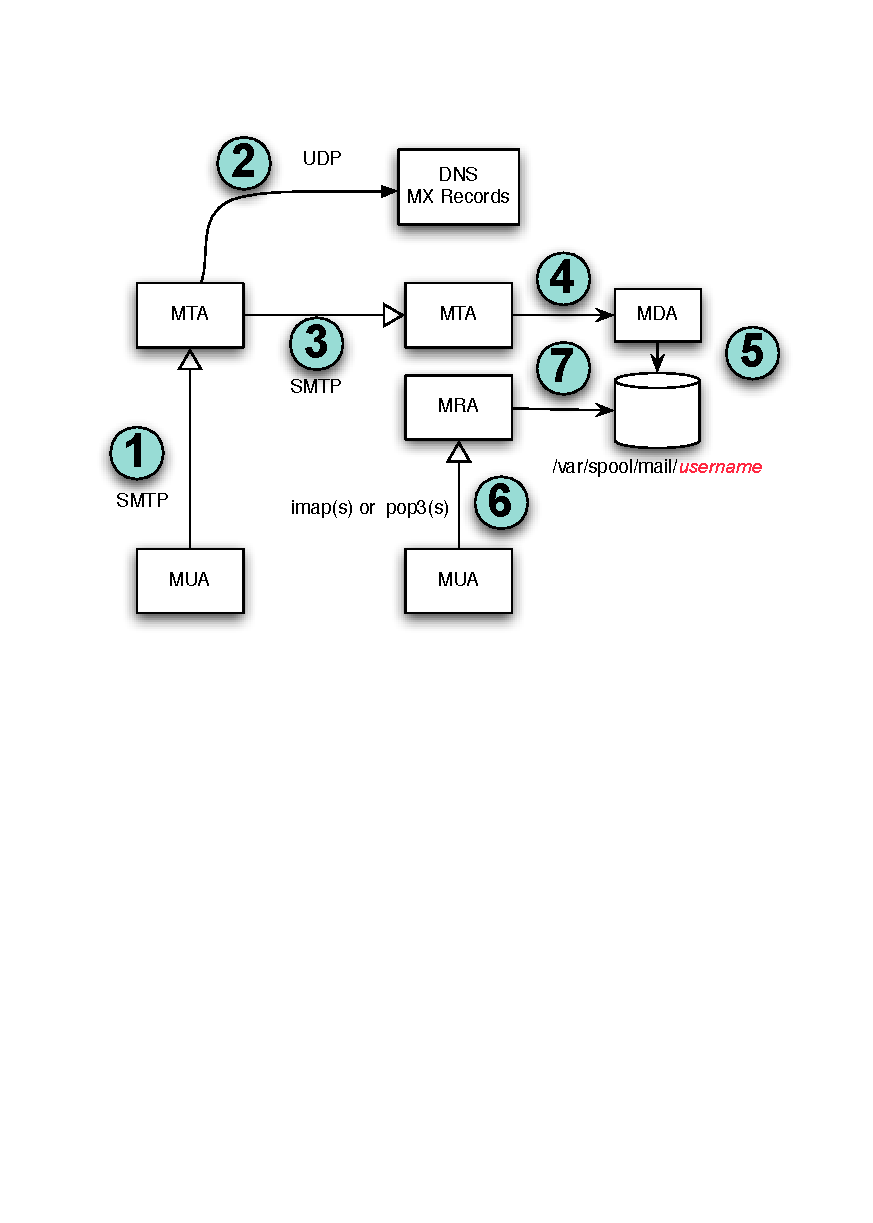
\includegraphics[scale=.8]{images/email-overview}


\end{frame} 
\subsection{smtp协议}


\begin{frame}{Simple Mail Transport Protocol(SMTP)}
\begin{itemize}
\item 和MTA交互的RFC标准协议

\begin{itemize}
\item 通常使用25号TCP端口
\item 扩展SMTP(ESMTP)提供了针对MTA的一些增强特性
\item MTA经常使用LMTP(Local Mail Transport Protocol)来和自己交互
\end{itemize}
\item 明文传送
\item MSP(Message Send Protocol) 例子

\begin{itemize}
\item mail -vs 'some subject ' \emph{username@localhost.localdmain}
\end{itemize}
\item 用telnet排查SMTP连接故障
\end{itemize}

\end{frame} 
\begin{frame}{SMTP协议的使用}
\begin{itemize}
\item SMTP协议命令

\begin{itemize}
\item HELO 通报来访者地址
\item MAIL FROM 发件人地址
\item RCPT TO 收件人地址
\item DATA 输入正文内容,用单独的.为行结束
\item QUIT 连线结束
\end{itemize}
\end{itemize}

\end{frame} 
\begin{frame}{安全与反垃圾邮件策略}
\begin{itemize}
\item 安全策略

\begin{itemize}
\item 拒绝从无法解析的域送来的邮件
\item 建立各种基于主机、用户、域的访问控制
\item 默认配置仅允许本地收发
\item 不再使用setuid的工具
\end{itemize}
\item 反垃圾邮件策略

\begin{itemize}
\item 默认情况下不做转发
\item 建立访问数据库
\item 检查邮件信头
\end{itemize}
\end{itemize}

\end{frame} 
\begin{frame}{Mail Transport Agent(MTA)}
\begin{itemize}
\item 系统默认提供两个MTA

\begin{itemize}
\item sendmail
\item postfix(缺省)
\end{itemize}
\item 通用特性

\begin{itemize}
\item 支持虚拟主机
\item 提供投递失败重试
\item 和spamassassin协作
\end{itemize}
\item 缺省访问控制

\begin{itemize}
\item sendmail/postfix没有setuid组件
\item 仅侦听在本地回路上
\item 转发禁止
\end{itemize}
\end{itemize}

\end{frame} 
\subsection{sendmail概述}

\begin{frame}{sendmail服务一览}

类型:SysV管理的服务

软件包:sendmail,sendmail-cf,sendmail-doc

守护进程:/usr/sbin/sendmail

脚本:/etc/init.d/sendmail

端口:25(smtp)

配置:/etc/mail/sendmail.mc,/etc/aliases,\ldots{}

相关:procmail(MDA),spamassassin,tcp\_wrappers


\end{frame} 
\subsection{sendmail配置}


\begin{frame}{sendmail 配置介绍}
\begin{itemize}
\item 使用和推荐m4 宏语言

\begin{itemize}
\item dnl <space> 表示注释
\end{itemize}
\item service sendmail restart 使用/etc/mail/Makefile

\begin{itemize}
\item /etc/mail/sendmail.mc转为/etc/mail/sendmail.cf
\item 重新hash多个文本数据库
\item make比较时间戳,可以touch一个文件来强制重建/重新hash
\end{itemize}
\item sendmail-cf 缺省并不安装
\item init脚本并不重建文件,除非安装了sendmail-cf软件包
\end{itemize}

\end{frame} 
\begin{frame}{sendmail 流入配置}
\begin{itemize}
\item 修改/etc/mail/sendmail.mc,侦听所有网络接口\\
dnl DEAMON\_OPTIONS(`Port=smtp,Address=127.0.0.1,Name=MTA')dnl
\item 服务器可能提及到的主机名都加入到/etc/mail/local-host-names里
\item 修改访问控制

\begin{itemize}
\item 跟新/etc/hosts.\{allow,deny\}
\item 增加防火墙规则,允许SMTP传输
\end{itemize}
\item 重启sendmail
\end{itemize}

\end{frame} 
\begin{frame}{sendmail 流出配置}
\begin{itemize}
\item 缺省配置 /etc/mail/submit.cf

\begin{itemize}
\item 几乎不要修改
\item 可以把sendmail当作客户端MSP
\end{itemize}
\item 伪装成域,而不是单个主机

\begin{itemize}
\item 取消/etc/mail/sendmail.mc下面几行的注释\\
EXPOSED\_USER(`root')dnl\\
FEATURE(masquerade\_envelope)dnl\\
MASQUERADE\_AS(`example.com')dnl\\
FEATURE(masquerade\_entire\_domain)dnl
\item 这些选项和带外地址重写结合一起工作
\end{itemize}
\end{itemize}

\end{frame} 
\begin{frame}{/etc/aliases}
\begin{itemize}
\item 定义本地用户的别名
\item 别名后的映射对象可以是:

\begin{itemize}
\item 一个本地用户
\item 多个本地用户(用逗号分隔)
\item 本地文件(需要指出路径)
\item 指令(需要管道)
\item 另一个email地址
\end{itemize}
\item 设定完/etc/aliases后,需要运行newaliases更新aliases.db
\end{itemize}

\end{frame} 
\begin{frame}{/etc/virtusertable}


\begin{itemize}
\item 允许在邮件服务中使用虚拟域及虚拟用户并自动映射:\\
joe@abc.com joe\\
@wenhua.org root@wenhua.org \\
eddy@msn.com eddy@wenhua.org
\end{itemize}

\end{frame} 
\begin{frame}{/etc/mail/access}
\begin{itemize}
\item 用于定义接受或拒绝的邮件来源:
\item 格式:\\
IP/域名 设定值
\item 设定值:

\begin{itemize}
\item REJECT:拒绝
\item OK:无条件接受
\item RELAY:允许转发
\item DISCARD:丢弃
\end{itemize}
\end{itemize}

\end{frame} 
\begin{frame}{带外(outbound)地址重写}
\begin{itemize}
\item 在/etc/mail/sendmail.mc里增加下面几行\\
FEATURE(genericstable)dnl\\
FEATURE(`always\_add\_domain')dnl\\
GENERICS\_DOMAIN\_FILE(`/etc/mail/local-host-names')dnl
\item 创建和填充/etc/mail/genericstable\\
paul@example.com paul@otherexample.com\\
david@example.com david.lastname@example.com
\item 域必须在/etc/mail/local-host-names列出
\item 地址重写只对SMTP有效,对LMTP无效
\end{itemize}

\end{frame} 
\begin{frame}{sendmail SMTP 限制}
\begin{enumerate}
\item 在/etc/mail/sendmail.mc里加入下面一行激活\\
FEATURE(`blacklist\_recipients')dnl
\item 在/etc/mail/access里加入限制:\\
From:90trialspammer@aol.com REJECT


Connect:spamRus.net REJECT


Connect:204.168.23 REJECT


Connect:10.3 OK


From:virtualdomain1.com RELAY


To:user@dom9.com ERROR:550 mail discarded


To:nobody@ ERROR:550 bad name

\end{enumerate}
\begin{itemize}
\item 使用标签(tag)来表明黑名单是对sender,recipient还是MTA有效
\item 没有标签的条目发对使用
\end{itemize}

\end{frame} 
\begin{frame}{sendmail 操作}
\begin{itemize}
\item /etc/mail/local-host-names

\begin{itemize}
\item 必须包含服务器主机名和别名
\end{itemize}
\item mail -v \emph{user}

\begin{itemize}
\item 查看本地转发的SMTP交换
\end{itemize}
\item mailq/mailq -Ac

\begin{itemize}
\item 查看将要将要投递的队列
\end{itemize}
\item sendmail -q

\begin{itemize}
\item 重新处理邮件队列
\end{itemize}
\item tail -f /var/log/maillog

\begin{itemize}
\item 实时查看日志
\end{itemize}
\end{itemize}


\subsection{postfix概述}


\end{frame} 
\begin{frame}{postfix服务一览}
\begin{itemize}
\item 类型:SysV管理的服务
\item 软件包:postfix
\item 守护进程:/usr/libexec/postfix/master,其他
\item 脚本:/etc/init.d/postfix
\item 端口:25(smtp)
\item 配置:/etc/postfix/mail.cf,其他
\item 相关:procmail
\end{itemize}

\end{frame} 
\subsection{postfix配置}


\begin{frame}{postfix配置介绍}
\begin{itemize}
\item /etc/postfix/main.cf

\begin{itemize}
\item 良好的注释,采取key=values对形式,按序出现在需要配置的地方
\item 一行开头的空白表示上一行的延续
\item 前面的是可以被作为后面key值序列的变量使用\\
key1=value1\\
key2=\$key1,value2
\end{itemize}
\item postconf

\begin{itemize}
\item 显示设置:postconf -d
\item 显示当前非缺省设置:postconf -n
\item 修改main.cf: postconf -e \emph{key=value}
\item 显示支持的映射类型: postconf -m
\end{itemize}
\end{itemize}

\end{frame} 
\begin{frame}{postfix 流入配置}
\begin{itemize}
\item 修改/etc/postfix/main.cf

\begin{itemize}
\item 监听在所有接口上\\
inet\_interfaces = all
\item 指定服务器可能参考的每一个主机名和别名\\
mydestination = \$myhostname, localhos.\$mydomain,localhost, \$mydomain
\end{itemize}
\item 增加防火墙规则,允许SMTP传输
\item 重启postfix
\item postfix 流出配置
\item 缺省配置提供

\begin{itemize}
\item postfix可以充当MSP客户端
\item 不再需要对单个主机做更多的配置
\item postfix自动解析本地主机名和域名
\end{itemize}
\item 伪装成域名

\begin{itemize}
\item myorigin = \$mydomain


masquerade\_exceptions = root

\end{itemize}
\end{itemize}

\end{frame} 
\begin{frame}{带内postfix别名}
\begin{itemize}
\item 本地别名 /etc/aliases,和sendmail一致
\item 虚拟别名

\begin{enumerate}
\item 在main.cf激活\\
virtual\_alias\_maps = hash:/etc/postfix/virtual
\item 在/etc/postfix/virtual定义,使用和sendmail(virtusertable)同样的格式
\item 重新hash文件: postmap /etc/postfix/virtual
\end{enumerate}
\end{itemize}

\end{frame} 
\begin{frame}{带外地址重写}
\begin{enumerate}
\item 在/etc/postfix/main.cf里激活

\begin{enumerate}
\item smtp\_generic\_maps = hash:/etc/postfix/generic
\end{enumerate}
\item 在/etc/postfix/generic定义\\
paul@example.com paul@otherexample.com\\
david@example.com david.lastname@example.com
\item 重新hash文件:postmap /etc/postfix/generic
\end{enumerate}

\end{frame} 
\begin{frame}{postfix 限制}
\begin{enumerate}
\item 创建/etc/postfix/access

\begin{itemize}
\item /etc/mail/access的无标签版本
\item 重新hash postmap /etc/postfix/access
\end{itemize}
\item 编辑main.cf\\
smtpd\_TAG\_restrictions =\\
check\_TAG\_access hash:/etc/postfix/access, \ldots{}

\begin{itemize}
\item TAG是sender,recipient,client中的一个
\item 例子\\
smtpd\_recipient\_restrictions =


check\_recipient\_access hash:/etc/postfix/access,


permit\_mynetworks, reject\_unauth\_destination

\end{itemize}
\end{enumerate}

\end{frame} 
\begin{frame}{postfix 操作}
\begin{itemize}
\item main.cf 设置

\begin{itemize}
\item 服务器名:mydestinatio 必须包含服务器的名字和别名
\item 监听接口:inet\_interfaces = all
\item 归档所有邮件:always\_bcc = \emph{address}
\end{itemize}
\item 查看SMTP交换:mail -v user@domain.tld
\item 查看延期的邮件:postqueue -p
\item 清空延期的邮件:postqueue -f
\item 实时查看日志:tail -f /var/log/maillog
\end{itemize}

\end{frame} 
\subsection{Procmail 概述}

\begin{frame}{Procmail,邮件投递代理(Mail Delivery Agent)}
\begin{itemize}
\item 不同的使用,包括

\begin{itemize}
\item 对收到来信进行排序,并送入不同目录或者文件
\item 预处理邮件
\item 邮件达到后,开启一个事件或者程序
\item 自动转发邮件给其他人
\end{itemize}
\item 激活 procmail

\begin{itemize}
\item sendmail:缺省激活
\item postfix:修改 /etc/postfix/main.cf\\
mailbox\_command = /usr/bin/procmail
\end{itemize}
\item 有可能在短时间内产生大量转发邮件,因此配置时应小心谨慎
\end{itemize}

\end{frame} 
\begin{frame}{Procmail和访问控制}
\begin{itemize}
\item 初始化控制

\begin{itemize}
\item Procmail以 nobody 帐号运行
\item Procmail属于 mail 组
\item /var/spool/mail 仅对 root 和 mail 组可写
\end{itemize}
\item 要求:改变procmail程序以setgid方式运行\\
chmod g+s \$(which procmail)
\end{itemize}

\end{frame} 
\subsection{procmail 配置}


\begin{frame}{procmail 配置介绍}
\begin{itemize}
\item 配置文件按序处理

\begin{enumerate}
\item /etc/procmailrc
\item \textasciitilde{}/.procmailrc
\end{enumerate}
\item 配置文件里的元素

\begin{itemize}
\item 指令: VERBOSE=yes
\item 变量:LOGFILE=/var/spool/mail/procmail.log
\item 处理

\begin{itemize}
\item 一行以':0'开始
\item 零或多个匹配行使用正规表达式
\item 一行或多行动作
\end{itemize}
\end{itemize}
\end{itemize}

\end{frame} 
\begin{frame}{Procmail 处理实例}
\begin{itemize}
\item 将来自wgzhao关于linux的邮件转发给lancy,并复制到linux目录\\
:0


{*}\textasciicircum{}From.{*}wgzhao


{*}\textasciicircum{}Subject:.{*}linux


\{ :0 c


! todd@xplore.cn


:0


linux


\}

\item man手册:procmailex,procmailrc,procmail
\end{itemize}

\end{frame} 
\subsection{邮件接收}


\begin{frame}{Mail Retrieval Protocols}
\begin{itemize}
\item 邮局协议 Post Office Protocols

\begin{itemize}
\item 所有的数据,包括密码,通过TCP 110端口明文传输
\item 使用POP3s对在TCP 995端口上传输的数据提供了SSL加密
\end{itemize}
\item 交互邮件访问协议 Internet Mail Access Protocol

\begin{itemize}
\item 所有的数据,包括密码,通过TCP 143端口明文传输
\item 使用POP3s对在TCP 993端口上传输的数据提供了SSL加密
\end{itemize}
\item Dovecot 支持POP3,POP3s,IMAP和IMAPs
\end{itemize}

\end{frame} 
\subsection{配置dovecot}


\begin{frame}{Dovecot服务一览}
\begin{itemize}
\item 类型:SysV管理的服务
\item 软件包:dovecot
\item 守护进程:/usr/sbin/dovecot
\item 脚本:/etc/init.d/dovecot
\item 端口:110(pop3),995(pop3s),143(imap),993(imaps)
\item 配置:/etc/dovecot.conf
\item 相关:procmail,fetchmail,openssl
\end{itemize}

\end{frame} 
\begin{frame}{Dovecot 配置}
\begin{itemize}
\item 缺省监听在所有的IPv6和IPv4接口上
\item 在/etc/dovecot.conf里指定协议

\begin{itemize}
\item protocols = imap imaps pop3 pop3s
\end{itemize}
\item 使用SSL之前创建私钥和自签名证书

\begin{enumerate}
\item 确认系统时间以免时钟问题
\item 检查/etc/dovecot.conf里配置密钥和证书的位置
\item 运行 make -C /etc/pki/tls/certs dovecot.pem

\begin{itemize}
\item 创建单个PEM文件同时包含密钥和证书
\end{itemize}
\item 拷贝新的PEM文件到定义密钥和证书的位置
\end{enumerate}
\end{itemize}

\end{frame} 
\begin{frame}{校验POP操作}
\begin{itemize}
\item 校验服务器操作

\begin{itemize}
\item 图形化工具:Thundbird,kmail,\ldots{}
\item 文字模式:mutt,fetchmail\\
mutt -f pop://user@server{[}:port{]}\\
mutt -f pops://user@server{[}:port{]}
\item 可以使用telnet(pop3)或者openssl s\_client (pop3s)
\end{itemize}
\end{itemize}

\end{frame} 
\begin{frame}{校验IMAP操作}
\begin{itemize}
\item 校验服务器操作

\begin{itemize}
\item 图形化工具:Thundbird,kmail,\ldots{}
\item 文字模式:mutt,fetchmail\\
mutt -f imap://user@server{[}:port{]}\\
mutt -f imaps://user@server{[}:port{]}
\end{itemize}
\item 也可以使用telnet(IMAP)或openssl s\_client(IMAPs)
\end{itemize}

\end{frame} 
\subsection{邮件服务实验}


\begin{frame}{实验I:配置sendmail为MTA}
\begin{description}
\item [{场景:}] 一个站点需要一个本地的邮件服务器来支持,域名为example.com。考虑安全实现
\item [{要求:}] 为example.com提供sendmail邮件服务
\end{description}
提示
\begin{enumerate}
\item 默认sendmail仅接受本地回路请求
\item 和DNS结合
\item 考虑防火墙
\end{enumerate}

\end{frame} 
\begin{frame}{实验II:迁移到postfix}
\begin{description}
\item [{场景:}] 使用sendmail的设备决定迁移到postfix来提供邮件服务。安装和实现它,适当考虑安全。
\item [{要求:}] 为example.com提供postfix邮件服务
\end{description}

\end{frame} 
\begin{frame}{实验III:增加新的别名}
\begin{description}
\item [{场景:}] 你的机构需要一一系列常用的email帐号,他们会重定向到实际用户帐号。使用邮件别名实现这个特性
\item [{要求:}] 邮件别名分布系统
\end{description}

\end{frame} 
\begin{frame}{实验IV:安装Dovecot作为MRA}
\begin{description}
\item [{场景:}] 远程用户需要访问在本地服务器上的邮件。配置Dovecot,允许所有邮件获取协议的连接,加密协议使用缺省证书。
\item [{要求:}] 配置MRA功能服务器
\end{description}
提示
\begin{enumerate}
\item 首先实现非加密协议的邮件获取
\item 后实现加密协议的邮件获取
\item 选择好的MUA或者命令行工具来调试
\end{enumerate}

\end{frame} 
\begin{frame}{实验V:创建唯一的Dovecot证书}
\begin{description}
\item [{场景:}] 对从非安全协议嗅探密码的担忧,决定使用特定站点的加密证书
\item [{要求:}] 实现MRA安全服务
\end{description}
提示
\begin{enumerate}
\item Dovecot 安装时,提供了通用的加密key,他们可能会遭遇中间人(man in the middle)攻击。
\item 考虑系统提供的key /etc/pki/tls/certs
\item make -C /etc/pki/tls/certs dovecot.pem
\end{enumerate}

\end{frame}

